%%
%% This is file `mcmthesis-demo.tex',
%% generated with the docstrip utility.
%%
%% The original source files were:
%%
%% mcmthesis.dtx  (with options: `demo')
%%
%% -----------------------------------
%%
%% This is a generated file.
%%
%% Copyright (C)
%%     2010 -- 2015 by Zhaoli
%%     2014 -- 2016 by Liam 
%%     2017 -- 2019 by Xuehan
%%
%% This work may be distributed and/or modified under the
%% conditions of the LaTeX Project Public License, either version 1.3
%% of this license or (at your option) any later version.
%%
%% This work has the LPPL maintenance status `maintained'.
%%
%% The Current Maintainer of this work is Xuehan.
%%
\documentclass{mcmthesis}
\bibliographystyle{IEEEtran}
\mcmsetup{CTeX = false,   % 使用 CTeX 套装时,设置为 true
        tcn = 2002134, problem = D,
        sheet = true, titleinsheet = true, keywordsinsheet = true,
        titlepage = true}
\usepackage{palatino}
\usepackage{mwe}
\usepackage{graphicx}
\usepackage{subcaption}
\usepackage{float}
\usepackage{multirow}
\usepackage{indentfirst}
\usepackage{gensymb}
\usepackage[ruled,lined,commentsnumbered]{algorithm2e}
\usepackage{geometry}

\begin{document}
\linespread{0.6} %%行间距
\setlength{\parskip}{0.5\baselineskip} %%段间距
\title{ti}

\date{\today}
	\begin{abstract}

	
		\begin{keywords}
		
		\end{keywords}
	\end{abstract}

\maketitle

\tableofcontents

\newpage

\section{Introduction}
\subsection{Problem Background}
	Football is one of the most well-known sports activities in the world.  The standard system of an 11-man football game is one goalkeeper and 10 players from each of the two teams. There are a total of 22 players who fight, defend and attack on the rectangular grass court.  The game scores by shooting the ball into the opponent's goal. When the game is over, the team with the most points wins.

	\begin{figure}[h]
		\centering
		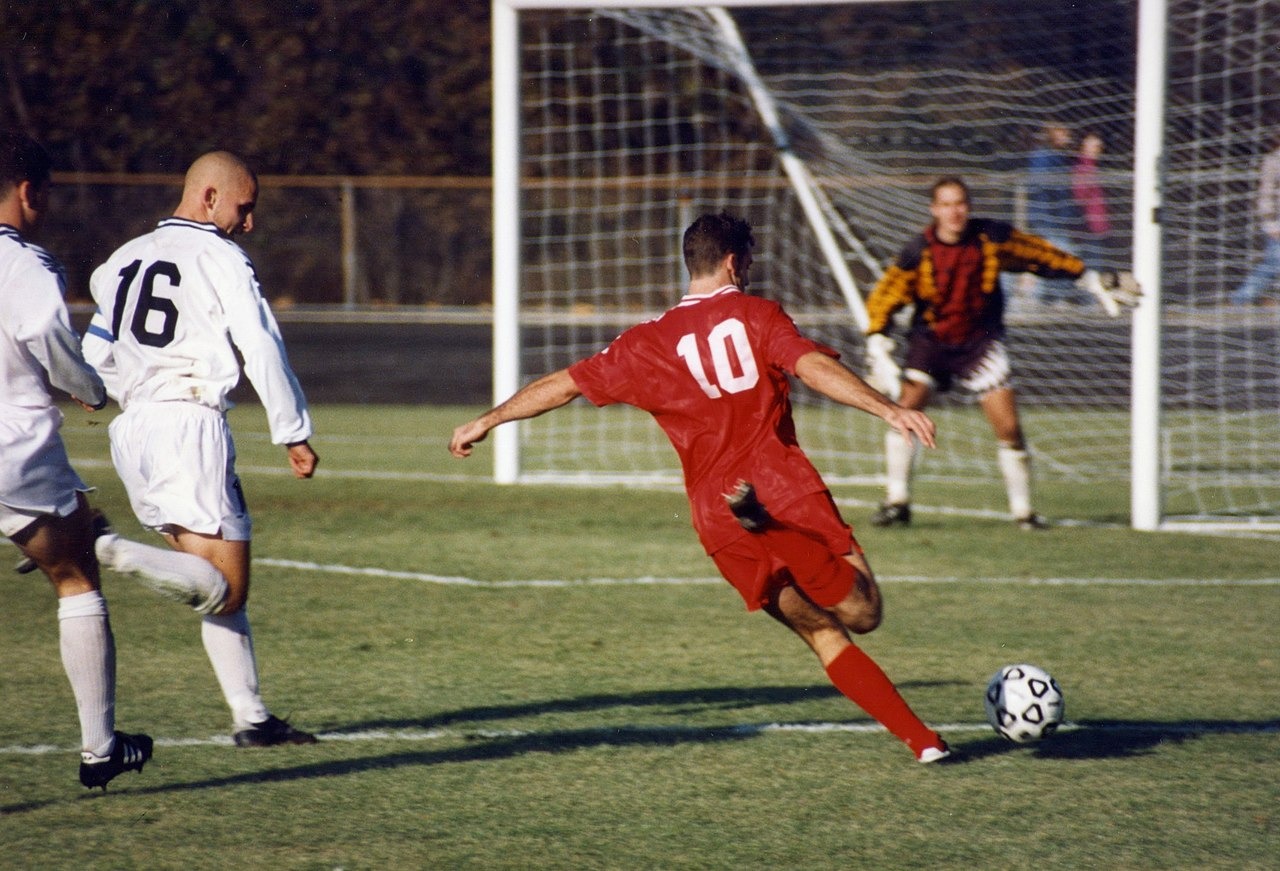
\includegraphics[width=0.75\textwidth]{figures/football.jpg}
		\caption{A Football Game~\cite{Wiki_Football}}
		\label{fig:football}
	\end{figure}

	As we all know, football is a sport that requires intense teamwork.  For it can show the importance of teamwork spirit more than superb personal ability.  Passing, as an offensive means that requires the cooperation of various players to play the biggest role, is just an important manifestation of the team spirit of football.  Therefore, to study the important role of teamwork in football, we will start by studying the passing network in football.

	Our goal is to build a network model to simulate the Huskies' passing network and study it.  Meanwhile, it is necessary to extract some representative parameters from the constructed network model.  Through the study of such parameters, we can accurately understand the team collaboration ability and structural characteristics of this team.
\subsection{Our Work}
	In this paper, we successfully built the Huskies' passing network model.  On the basis of this network model, we obtained some important parameters. In this way, we analyzed the team collaboration ability of the Huskies players, and offered some suggestion for its future structural strategy.

	In Section 2, we state some basic assumptions.  Section 3 contains the nomenclature used in the statement of our model.  Section 4 provides sufficient details about our network model.  Section 5 carries on the simulation experiment and analysis to our proposed model.  Section 6 provides some advice on its structural strategies for the Huskies.  Finally, we further analyze the sensitivity, advantages and disadvantages of our model in Section 7, and we obtain some conclusions on how to improve the teamwork spirit of general teams in Section 8.
\section{Assumptions}
	Our model is based on these following basic assumptions:
	\begin{enumerate}
		\item The average position of a player over a period of time is equivalent to the average of the position of the player in all events that occurred during that period.
		\item We consider a dyadic configuration tight if this kind of dyadic configuration appears far more often than others.  The same is true for triadic configurations.
	\end{enumerate}
\section{Nomenclature}
	Symbols that our model mainly uses are listed in Table \ref{tab:Nomen}.  Other symbols that are used only once will be described in the following chapters.
	\begin{table}
    	\centering
    	\caption{Nomenclature}
		\label{tab:Nomen}
		\begin{tabular}{c c}
			\hline	
				Symbol & Definition\\
			\hline
				$\textbf{A}$ & Football passing matrix\\
				$\textbf{B}$ & Adjacency matrix\\
				$G$ & Undirected graph representing the football passing network\\
				$p_{i}$ & The \emph{i}th player in Huskies\\
				$p_{ij}$ & Number of passes from player $i$ to player $j$\\
				$\langle$$X$$\rangle$ & The x-coordinate of the network centroid\\
				$\langle$$Y$$\rangle$ & The y-coordinate of the network centroid\\
				$D$ & The dispersion of the position of the players around the network centroid\\
				$r$ & The advance speed\\
			\hline
   	 	\end{tabular}
	\end{table}

\section{The Basic Model}
	In this section we will discuss our network model in detail.  First of all, we will begin with the establishment of our network model.  Then we will use our model to identify some patterns of the network.  Finally, we will also investigate the indicators of teamwork. 
\subsection{Build of the Network}
	First of all, we define Huskies' football passing matrix $\textbf{A}$.  When the number of players who have played is $n$, $\textbf{A}$ is a square matrix of $n \times n$, which is defined as:
	\begin{equation}\label{eq:Mat_A}
		a_{ij} =
		\begin{cases}
			p_{ij}& \text{$i \neq j$}\\
			0& \text{$i = j$}
		\end{cases}
	\end{equation}
	In this way, we obtain an asymmetric square matrix of order $n$.  Next, on this basis, we try to build an undirected graph model to describe the team's passing network.  But as we have mentioned before, the adjacency matrix of an undirected graph is a symmetric matrix, while the football passing matrix $\textbf{A}$ we constructed is asymmetric.  Therefore, we need to construct a symmetric adjacency matrix $\textbf{B}$ using this asymmetric passing matrix $\textbf{A}$.  To achieve this, we define $\textbf{B}$ as the sum of $\textbf{A}$ and the transposed matrix of $\textbf{A}$, that is to say, for each element $b_{ij}$ in B, the following formula is satisfied:
	\begin{equation}
		\label{eq:Mat_B}
		b_{ij} = a_{ij} + a_{ji}
	\end{equation}
	Now we can easily find that $\textbf{B}$ is equal to its transpose matrix.  Hence $\textbf{B}$ is a symmetric matrix.

	After getting $\textbf{B}$, we can continue to study the undirected graph $G$.  From the previous definition of the adjacency matrix, it can be seen that the nodes in this undirected graph represent the Huskies players, and the edges represent interactions between players.  For quantitative research, we define the weight of node $i$ in the undirected graph $G$ as the sum of the number of passes and catches by player $i$, and the weight of edge $E (i, j)$ is defined as the sum of the number of passes from player $i$ to player $j$ and the number of passes from player $j$ to player $i$.
	
	In order to have an intuitive understanding of the football passing network, we can draw this undirected graph on a schematic diagram of a football field.  Among them, circles represent nodes, and straight lines connecting circles represent edges.  For a node, the larger its size and the darker its color, the greater the weight of the node.  For an edge, the thicker its thickness and the darker its color, the greater the weight of the edge.  In addition, in order to gain a clear understanding of the formation and other factors of this team, we plot the nodes on the represented player's the average position in the studied period.  In this way, we obtain a schematic diagram which can intuitively reflect the football passing network.  Figure \ref{fig:playground} is an example by us.
	
	\begin{figure}[h]
		\centering
		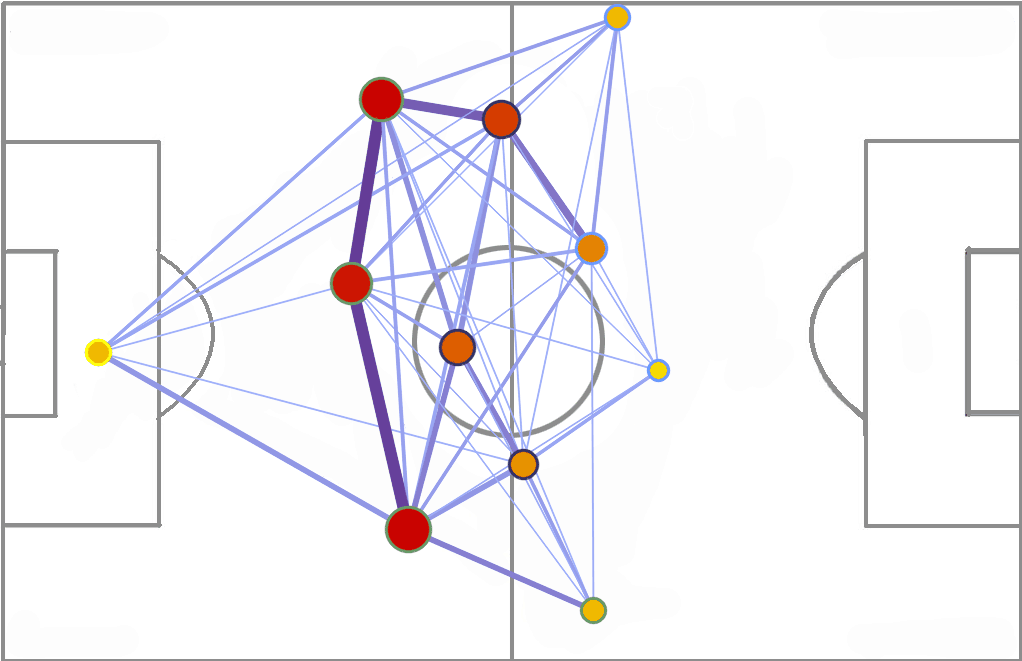
\includegraphics[width=\textwidth]{figures/playground.png}
		\caption{An Example of the Football Passing Network}
		\label{fig:playground}
	\end{figure}
\subsection{Identify Network Patterns}
	After establishing the football passing network, we will use this model to identify some special patterns of Huskies' network.  In the following chapters, we will investigate Huskies' continuous football passing chain, network centroid and advance speed to identify its patterns on multiple scales. 
\subsubsection{Continuous Football Passing Chain}
	Just as we have stated in assumption 2, when players in a dyadic or triadic configuration continuously pass each other far more frequently than they do with other players in the team, we consider this configuration tight.  Therefore, when investigating the tightness of such configurations, we need to study the behavior of continuous passing between players.  For this reason, we construct a continuous football passing chain as a tool to study this behavior according to the football passing network.

	In football games, passing is a very continuous activity.  It can be said that before occasion like shooting, out of bounds or the football is intercepted by the opposing player occurs, the passing can build a transitive binary relationship between our players.  Therefore, we can use this characteristic to construct a continuous football passing chain, which is continuous and transitive.  The general construction method is: According to the data in passingevents, we record the process of continuous passing of football between Huskies players with a linked chain.  This chain will continue until disruptive occasions such as shooting, out of bounds or the football is intercepted by the opponent occur.  In this way, we get a chain that records the continuous passing of the Huskies players.

	From the continuous football passing chains, we can easily identify those tight dyadic and triadic configurations.  For example, if we want to identify a dyadic configuration, we can study these chains based on the characteristics that players in this dyadic configuration pass each other more frequently.  We can just number these two players we are studying as 0 and 1. In this way, there will be a large number of fragments like"0 - 1 - 0 - 1" or "0 - 1 - 0 - 1 - 0" in the continuous football passing chain.  If we want to identify those triadic configurations that are tight, we can just look for those fragments such as "0 - 1 - 2 - 1" or "0 - 1 - 2 - 0" from the continuous football pass chain.  Obviously, we can make similar judgments about multiple configurations.  Therefore, it will be convenient for us to find out which kind of configuration appears most.
\subsubsection{Network Centroid And Advance Speed}
	Studying the network centroid and advancing ratio of Huskies' football passing network will display the spatial features of the network better~\cite{First}.  In this section, we will study the coordinates of the network centroid of the football passing network constructed previously, the dispersion of the position of Huskies players around the network centroid, and the advance speed.

	We first study the coordinates of football passing network centroid.  According to the description of coordinates in readme, the x-coordinate on the field is oriented from the perspective of the team that is attacking, where 0 indicates the attacking team's own goal, and 100 indicates the oppositing team's goal.  While for y-coordinate, 0 indicates the attacking team's left-hand side, and 100 indicates its right-hand side.  We define the coordinates of a pass $(x_{i}, y_{i})$ as the average of the origin and destination positions.  Furthermore, we define the coordinates of the network centroid over a period of time as the average coordinates of all passes during that period.  It can be expressed as the following formula: 
	$$\langle X \rangle=\sum_{i=1}^n\frac{1}{n} x_{i}$$
	$$\langle Y \rangle=\sum_{i=1}^n\frac{1}{n} y_{i}$$
	The change of the network centroid coordinates over time can clearly reflect the overall movement tendency of the entire team during this time.  Besides,regardless of the length of the research period, it can always convey some information about the spatial features of the network.

	Then we continue to study the dispersion of the position of Huskies players around the network centroid.  Similarly, we define the dispersion of the position of Huskies players around the network centroid over a period of time $D$ as the variance between the average position of each player and the position of the network centroid during this period.  It can show how dispersed the team is on the court during this time.  Hence it can also reflect the degree of team control over the playing field during this time.  The greater the degree of dispersion, the stronger the team's ability to control the field.

	Finally, we define the team's advance speed over a period of time $r$ as the ratio of the sum of the absolute values ​​of the lateral displacement and the sum of the absolute values ​​of the longitudinal displacement of all its passes during that period. Its formula is:
	$$r=\frac{|\Sigma \Delta x|}{|\Sigma \Delta y|}$$
	The advance speed indicates the team's passing direction.  Besides, it can also reflect the team's movement tendency and offensiveness during this period.
\subsection{Identify Teamwork Indicators}
	In this part, we comprehensively use AHP analysis method for modeling, and use judgment matrix to choose the weight of each factor. Besides, all scores are normalized before weighting.

	We comprehensively analyze the composition of events on the court and abstract based on existing data, and propose the following model.  The model that captures structural, configurational, and dynamical aspects of teamwork mainly includes the following five aspects:
	\begin{itemize}
		\item Offensive score;
		\item Defensive score;
		\item Coordination score;
		\item Robustness score;
		\item Flexibility score.
	\end{itemize}
\subsubsection{Offensive Score}
	In theory, tactics do not have the so-called advantages and disadvantages. The quality of tactics should depend on whether they can work wonders.  Based on this, the evaluation of an offensive tactic should be based on the performance of the attacker, the performance of the defender, and some special situations.
	\begin{enumerate}
	\item The Performance of the Attacker
	
	The offense on the football field is nothing more than passing and shooting. Apart from cases that the player can shoot alone because of excellent personal strength, good offense should be the result of successful teamwork.  Therefore, the number of passes should be the main consideration. Pass is divided into simple pass, smart pass, head pass, high pass and hand pass. And the main ones that appear in the offense are simple pass and smart pass. Head pass and high pass will only appear in specific situations, so they are not considered here.

	At the same time, the ball possession rate in the opponent's penalty area is also an important indicator of the aggressiveness of the offense. As the defender's last area, the penalty area is unquestionably strong.  Defensively, every striker will be pressed by at least one person.  And there will even be double-jacketing and multiple-jacketing situations.Therefore, the statistics of the ball control rate here is of great significance. It can comprehensively reflect the quality of tactics.Good tactics should be those the team can still control the ball in the face of high-intensity defense.

	And for the opponent will defend for each attack, the perfect attack should be that pass more to minimize the confrontation, so the number of confrontations in each attack should also be considered.  Note that each confrontation in the event table occurs in pairs: ground attacking duel and ground defending duel.  Therefore, this pair is directly referred to as ground duel in our analysis.  But in the event statistics, as long as the offensive and defensive opponents face each other, the situation is counted as ground duel.  Hence the events after the ground duel should be counted. The general choice is to quickly pass the ball to others or choose to pass the ball by himselt with extraodinary skills, so these two indicators should be considered together.

	Then good tactics also have the option of making fouls. Making fouls in the penalty area can earn a free kick. At this time, the foul is really worth a thousand dollars, so we will also count the number of fouls in each attack.
	
	Based on this, the quantitative indicators are as follows:
	
	\begin{itemize}
		\item $\eta$ is the football possession time ratio;
		\item $p_{1}$ is the number of simple passes;
		\item $p_{2}$ is the number of smart passes;
		\item $n_{1}$ is the number of passes after ground duel;
		\item $n_{2}$ is the number of ground duels after ground duel;
		\item $n_{3}$ is the number of free kicks after making the opponent foul.
	\end{itemize}

	The corresponding judgment matrix is:
	\begin{equation}\label{mat:1}
		M_{1}=
 	\begin{matrix}
   		 & \eta & p_{1} & p_{2} & n_{1} & n_{2} & n_{3} \\
   		\eta & 1 & 3 & 1 & 1 & 1 & \frac{1}{2} \\
		p_{1} & \frac{1}{3} & 1 & \frac{1}{3} & \frac{1}{3} &\frac{1}{3} &\frac{1}{7}\\
		p_{2} & 1 & 3 & 1 & 1 & 1 & \frac{1}{2} \\ 
		n_{1} & 1 & 3 & 1 & 1 & 1 & \frac{1}{2} \\ 
		n_{2} & 1 & 3 & 1 & 1 & 1 & \frac{1}{3} \\
		n_{3} & 2 & 7 & 2 & 2 & 3 & 1 
		
  	\end{matrix} 
	\end{equation}
	
	\item The Performance of the Defender
	
	The quality of an offense can also be judged from the other side, that is, the performance of the defensive end. The execution of an offensive tactic in place should theoretically fly the ball towards the goal and no opponent player blocks it.  At this time, the opponent team can only rely on the goalkeeper's response to try a save attempt.  Therefore, the defensive save attempt can also judge the quality of an offensive tactic.

	\begin{itemize}
		\item $d$ is the number of the opponent's save attempts.
	\end{itemize}

	\item Special Situations
	
	In some special cases, the tactics are just the front pavement. At that time, whether the goal can be achieved depends on the player ’s personal play and a certain degree of luck. In that case, it is usually a long corner kick, cross to the penalty area and rely on the player's aerial confrontation to pass the header, or run to the ball in advance to grab the ball and successfully shoot. In these cases, the tactics generally only prepare the first half, so it should be considered.

	\begin{itemize}
		\item $f$ is the number of shots right after crossing to the penalty area or right after corner.
	\end{itemize}

	\end{enumerate}
	The offensive tactics are scored by analyzing \textbf{the overall performance of the attacker, the performance of the defender, and the special situation}.The corresponding judgment matrix is:

	\begin{equation}\label{mat:2}
		M_{2}=
	  \begin{matrix}
		& M_{1} & d &f\\
   		M_{1} & 1 & 1 & 2 \\
   		d & 1 & 1 & 2 \\
   		f & \frac{1}{2} & \frac{1}{2} & 1
  	\end{matrix}
	\end{equation}
	
\subsubsection{Defensive Score}
	For the event table cannot reflect the occupancy of each defensive player, there is no way to know which defensive strategy is actually used. Therefore we can only start from the event-driven and consider the location of each event to establish our model.
	\begin{enumerate}
	\item ODC
	
	ODC refers to the number of opponent's successful passes within 20 yards of Huskies' bottom line. This area is the core defense area and the last defense area for each team.  By judging the number of successful passes by the opponent within 20 yards of the bottom line, it can clearly reflect the level of the team's defensive level from the side, and it can also reflect the level of the team's defensive tactics. Good defensive tactics will make it impossible for the enemy players to find a point to cope with, which means that the number of successful passes will be reduced.

	Therefore, the smaller the ODC value, the better the defensive effect of this game. Limiting the opponent's offense can indicate that the defensive quality is great, and the frequency of threats to the defensive area of ​​this team's own side is low.

	\begin{itemize}
		\item $ODC$ is the number of successful passes within 20 yards of this team's own baseline.
	\end{itemize}

	\item PPDA
	
	In PPDA, defensive actions are defined in the following four areas: steals, interceptions, confrontations, and fouls.  In this indicator, we only consider the pressure exerted by the player when defending against the opponent, and not care about other issues.

	The smaller the value of PPDA, it means that the team's defensive strength is higher, and this also shows from a side that in this particular area, the chances of the offensive team wanting to use the pass to tear the defensive team's defense line are relatively small.

	Of course, it is impossible for any team that adopts pressure defense to adopt such a strategy throughout the entire game. Most of the time, pressure defense has a trigger point, such as a player entering a specific area (this is also called trigger switch).  However, if all these factors are taken into account, the project volume will be quite huge, and some artificial subjective factors will be mixed into it.  Therefore, in the "defense strength" indicator, we will only provide an objective data, which is measured by all the defensive actions and the number of passes of the two sides in a specific area.

	\begin{itemize}
		\item $PPDA$ is total number of offensive passes $\div$ total number of defensive moves by the defending team.
	\end{itemize}

	\item The opponent's Shot/Goal
	
	From the macro level, measuring the defensive strength of a team will undoubtedly start from the number of broken goals.  However, the number of shots alone is not statistically significant. Therefore, the total number of shots of the enemy should also be counted. The shot / goal ratio is more general. It represents how many shots are required for each shot. The greater the number,  It means that the stronger the defense, the more difficult it is for enemy players to find good shots, and the stronger the defense of our players.

	\begin{itemize}
		\item $SG$ is the number of opponent's shot $\div$ the number of opponent's goal.
	\end{itemize}

	\end{enumerate}
\subsubsection{Coordination Score}
\subsubsection{Robustness Score}
\subsubsection{Flexibility Score}
\section{Implementation}
	In this section, we will analyze network patterns and teamwork indicators of Huskies' football passing network by studying the data given in problem. 
\subsection{Network Patterns}
	We will search for the dyadic and triadic configurations that often appear by studying continuous football passing chain first.  After that, we will analyze the spatial features of Huskies by investigating the network centroid and advance speed.
\subsubsection{Dyadic And Triadic Configuration}
	In a directed graph, we call different connection methods in dyadic and triadic configurations as different mode motifs.  It is obvious that dyadic and triadic configurations both have multiple different mode motifs~\cite{Second}.  In order to make statistics on these different mode motifs and determine which one appears most, we need to further visualize the continuous football passing chain.  Our idea is to reconstruct the continuous football pass chain into the form of a directed graph, so that the number of occurrences of motifs can be identified from the graph according to different directed graphs corresponding to different mode motif.

	First, we store the data given in the problem into a continuous football passing chain in the form of a linked list.  After that, we correspond the continuous football pass chain with the players to construct a directed continuous football pass graph.  Now, we can identify those frequently appearing mode motifs from these directed graphs.  We have made statistics on the occurrence of different mode motifs, and the results are shown in the following figures.

	\begin{figure}[h]
		\centering
		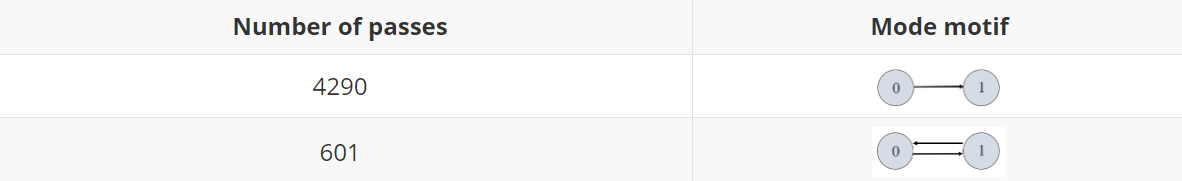
\includegraphics[width=0.75\textwidth]{figures/motif2.png}
		\caption{Statistics on the Occurrences of Different Mode Motifs of Dyadic Configuration}
		\label{fig:motif2}
	\end{figure}
	\begin{figure}[h]
		\centering
		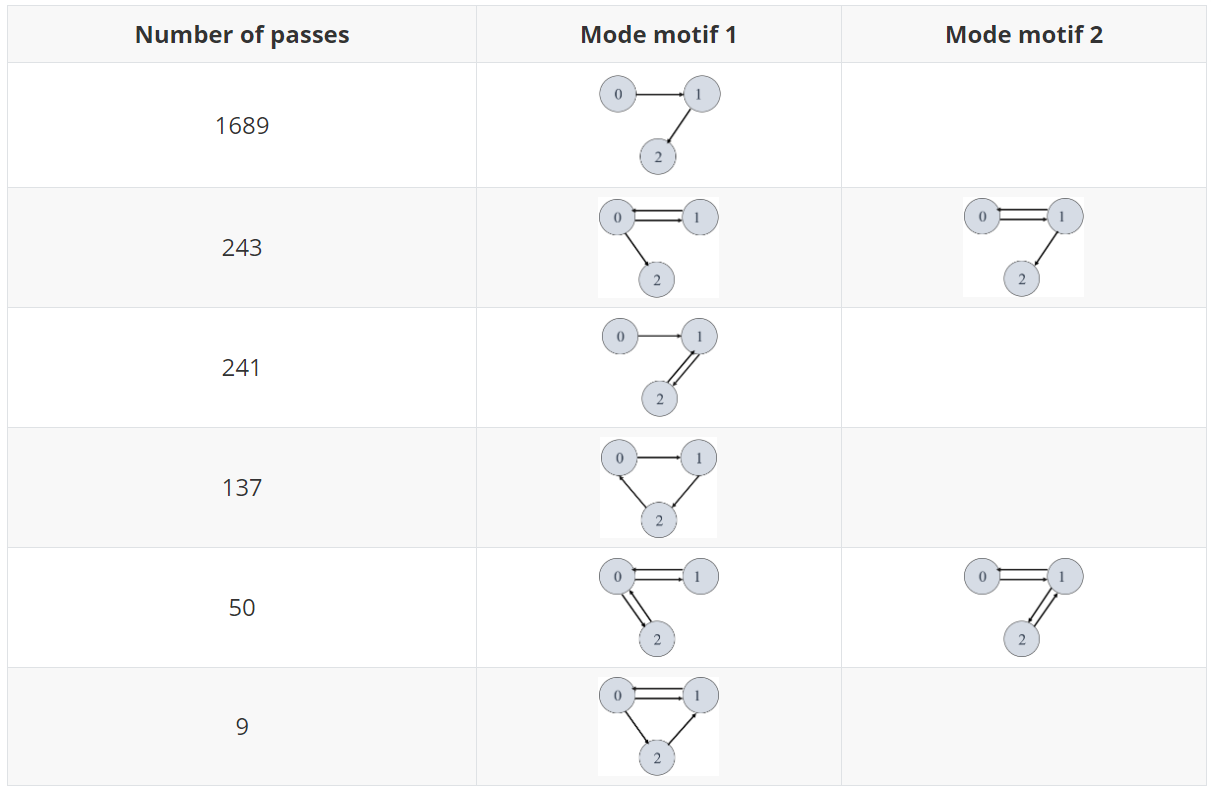
\includegraphics[width=0.75\textwidth]{figures/motif3.png}
		\caption{Statistics on the Occurrences of Different Mode Motifs of Triadic Configuration}
		\label{fig:motif3}
	\end{figure}
	
	We ignore the naive case that appears first in each configurations.  From figure \ref{fig:motif2} and figure \ref{fig:motif3}, we can intuitively see that in the case of dyadic configurations, the Huskies often use "0 - 1 - 0" and "0 - 1 - 0 - 1" mode motifs for passing.  For the triadic cases, it often uses "0 - 1 - 0 - 2", "0 - 1 - 2 - 1" and "0 - 1 - 2 - 0" mode motifs.  Compared with the longer dyadic and triadic chains, these passing mode motifs have more flexibility, but  can still be improved.

	In addition to dyadic and triadic configurations, we also select the case where the number of players is 4 as a representative of multiple configurations, and make statistics on the occurrence of its different mode motifs.  But because its number of mode motifs is far more than dyadic and triadic configurations, we put it in the appendices.
\subsubsection{Spatial Features}
	In this part, we have calculated the coordinates of the network centroid, the dispersion of the position of the players around the network centroid and advance speed of the Husky team's football passing network.  In order to make the results more general, we have calculated both the changes of these statistics per minute in a game, and the changes of these quantities in different games throughout the season.  Here are our statistics.

	We will analyze the statistics of a game first. Figure \ref{fig:game} shows the statistics of Huskies in a certain game.  From the coordinates of the network centroid, it can be seen that the Huskies players were closer to the opponent's goal in the second half, reflecting their fierce offensive in the second half.  It is clear by investigating the dispersion of the position of the players around the network centroid that the players are more concentrated in the second half, which confirms the opinion that the offensive in the second half is more fierce.  Judging from the advance speed, as the game progresses, the movement of the Huskies players is more inclined to go straight to the goal instead of a roundabout movement, which also confirms the previous opinion.
	\begin{figure}[h]
		\centering
		\begin{subfigure}[b]{0.5\textwidth}
			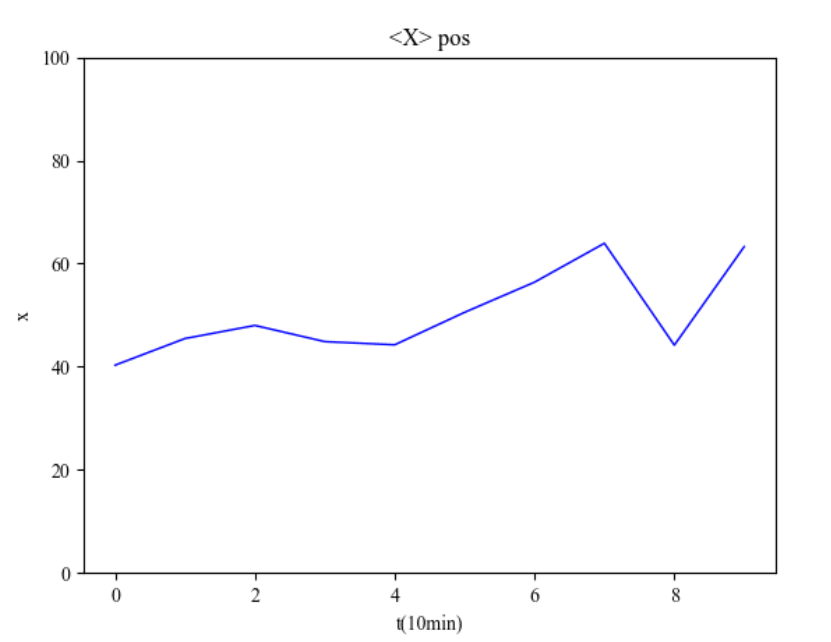
\includegraphics[width=\textwidth]{figures/xc1.png}
			\caption{The X-coordinate of the Network Centroid.}
			\label{fig:x1}
		\end{subfigure}%
		\begin{subfigure}[b]{0.5\textwidth}
			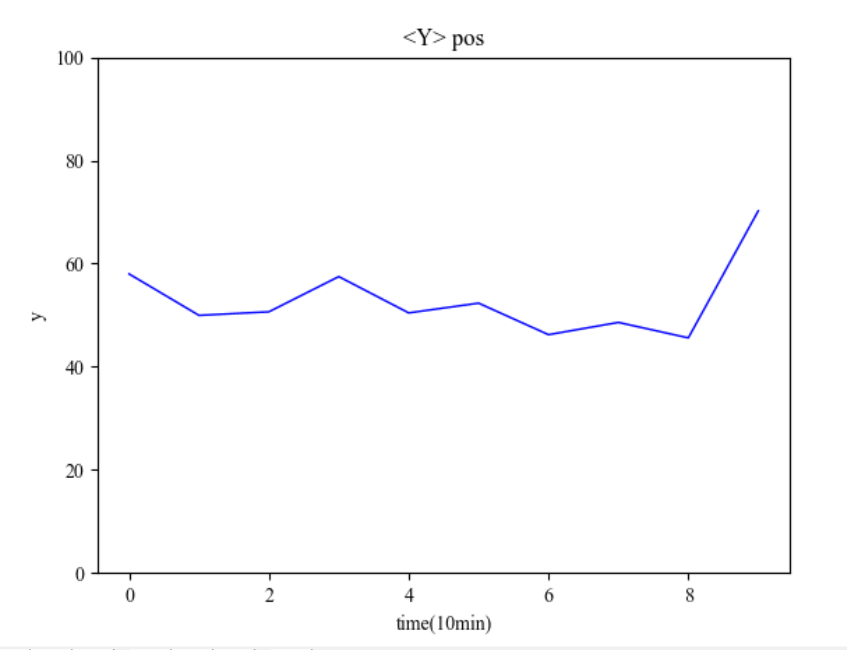
\includegraphics[width=\textwidth]{figures/yc1.png}
			\caption{The Y-coordinate of the Network Centroid.}
			\label{fig:y1}
		\end{subfigure}
		\begin{subfigure}[b]{0.5\textwidth}
			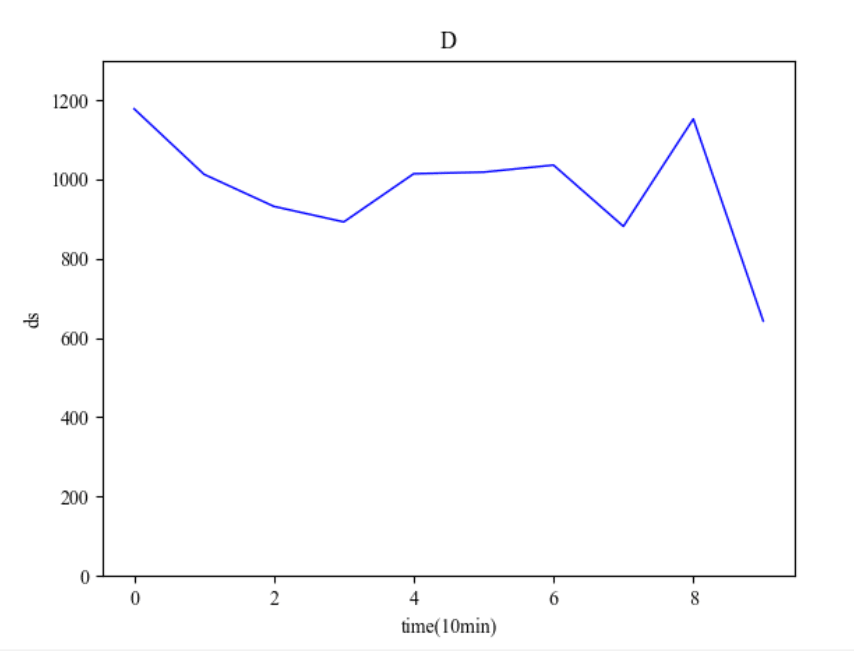
\includegraphics[width=\textwidth]{figures/d1.png}
			\caption{The Dispersion of the Position of the Players.}
			\label{fig:d1}
		\end{subfigure}%
		\begin{subfigure}[b]{0.5\textwidth}
			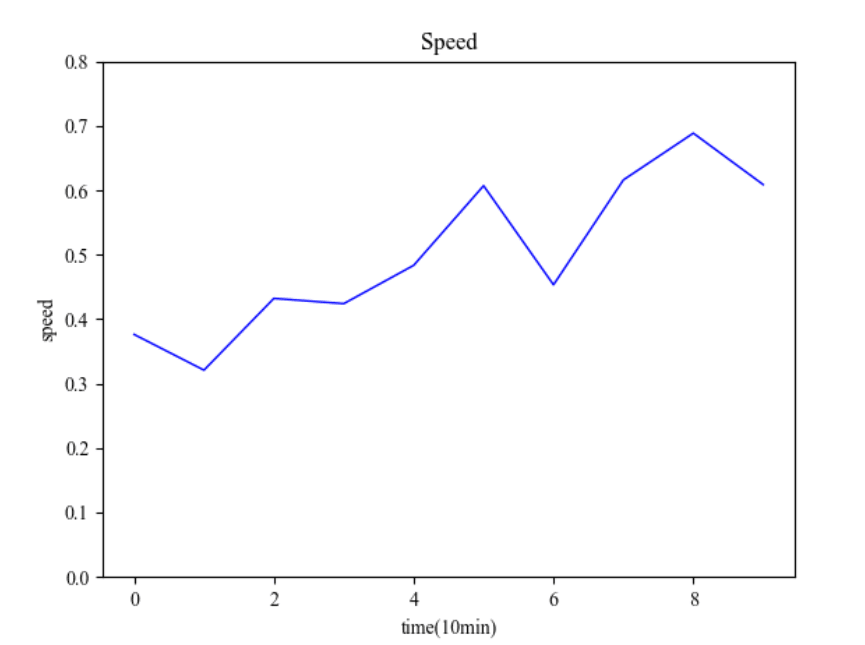
\includegraphics[width=\textwidth]{figures/s1.png}
			\caption{The Advance Speed.}
			\label{fig:s1}
		\end{subfigure}
		\caption{The Change of Network Centroid's Coordinates, the Dispersion of the Position of the Players around the Network Centroid And the Advance Speed over Time in a Game.}\label{fig:game}
	\end{figure}

	After that, we can also analyze the changes in the spatial features of the Huskies players throughout the entire season.  It can be seen from Figure \ref{fig:season} that the coordinates of the network centroid are fluctuating throughout the season, but the amplitude of the fluctuations is not very large. It can be considered that the average spatial position of the Huskies players is relatively stable in all games throughout the season.  The change of thedispersion of the position of the players around the network centroid and advance speed throughout the season is more obvious, indicating that the spatial distribution density of the Huskies players and the direction of passes will make relatively clear changes with different opponents.

	\begin{figure}[h]
		\centering
		\begin{subfigure}[b]{0.5\textwidth}
			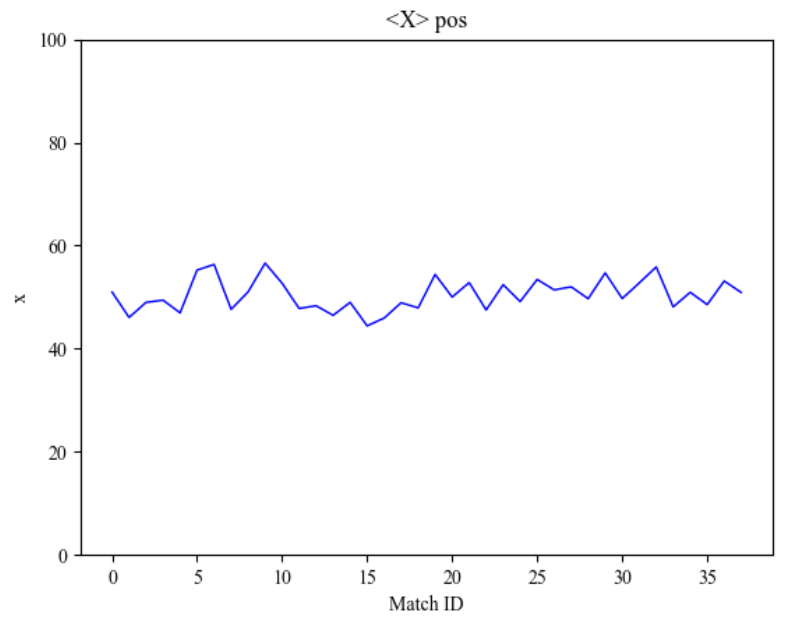
\includegraphics[width=\textwidth]{figures/xc2.png}
			\caption{The X-coordinate of the Network Centroid.}
			\label{fig:x2}
		\end{subfigure}%
		\begin{subfigure}[b]{0.5\textwidth}
			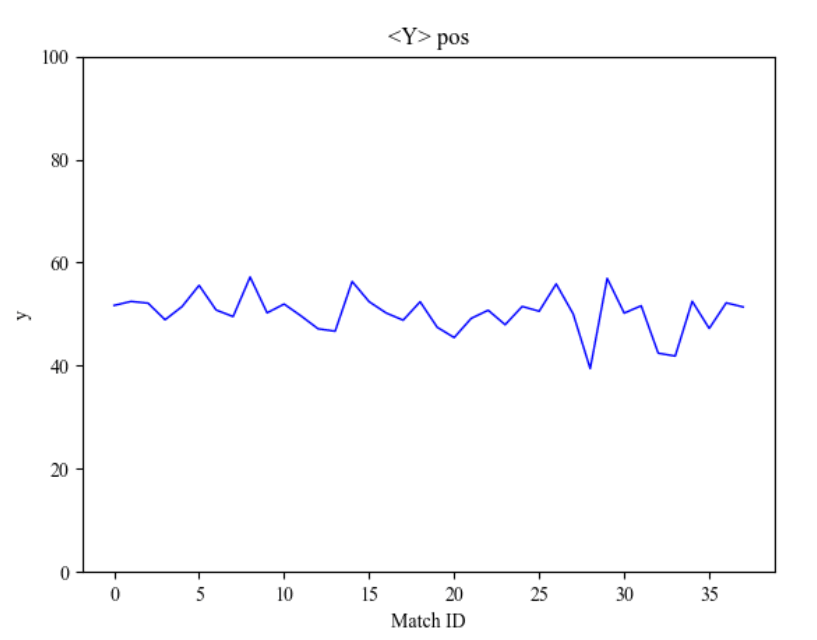
\includegraphics[width=\textwidth]{figures/yc2.png}
			\caption{The Y-coordinate of the Network Centroid.}
			\label{fig:y2}
		\end{subfigure}
		\begin{subfigure}[b]{0.5\textwidth}
			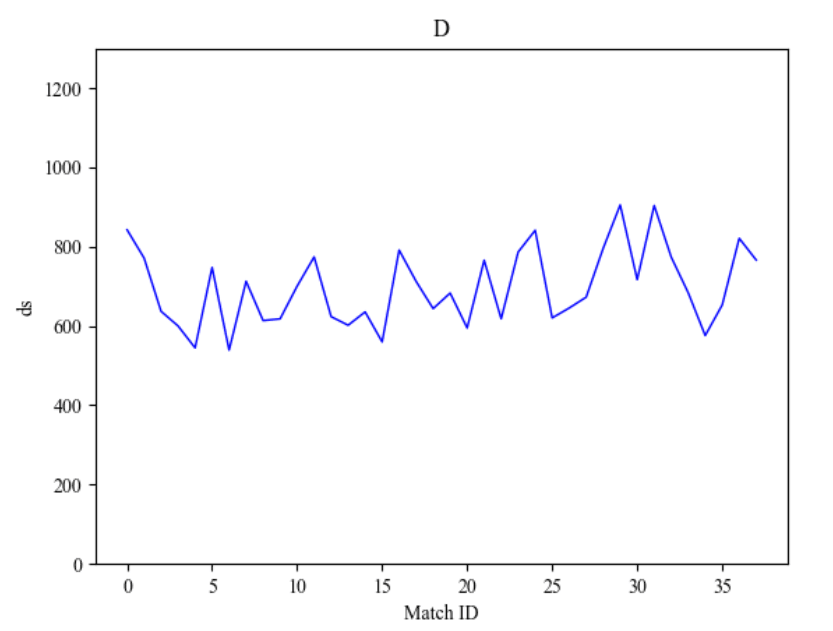
\includegraphics[width=\textwidth]{figures/d2.png}
			\caption{The Dispersion of the Position of the Players.}
			\label{fig:d2}
		\end{subfigure}%
		\begin{subfigure}[b]{0.5\textwidth}
			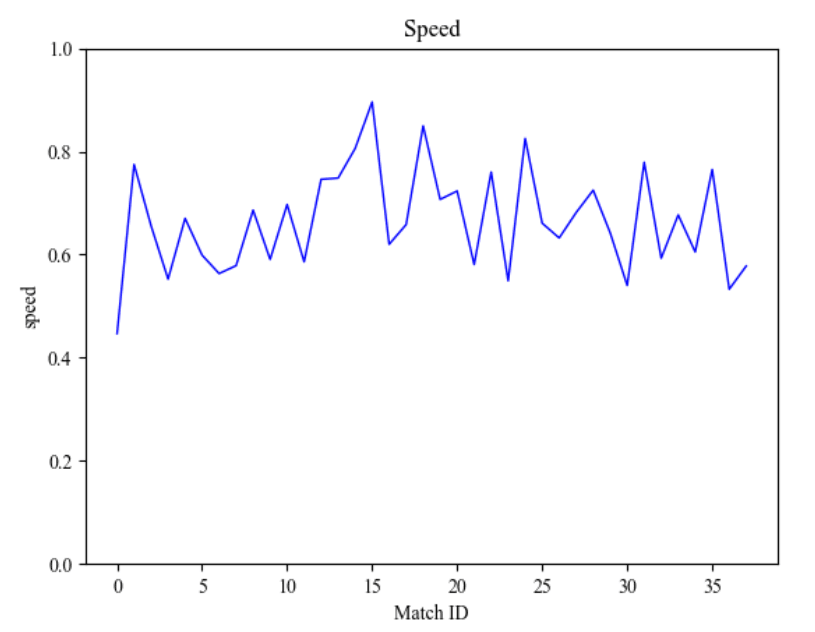
\includegraphics[width=\textwidth]{figures/s2.png}
			\caption{The Advance Speed.}
			\label{fig:s2}
		\end{subfigure}
		\caption{The Change of Network Centroid's Coordinates, the Dispersion of the Position of the Players around the Network Centroid And the Advance Speed over Games in the Entire Season.}\label{fig:season}
	\end{figure}
\subsection{Teamwork Indicators}
\section{Structural Strategies}
\section{Model Analysis}
\subsection{Sensitivity Analysis}
\subsection{Strengths and Weakness}
\section{Conclusion}

\bibliography{ref}
\newpage

\begin{appendices}

\section{Mode Motifs for Multiple Configurations}

\begin{figure}[h]
	\centering
	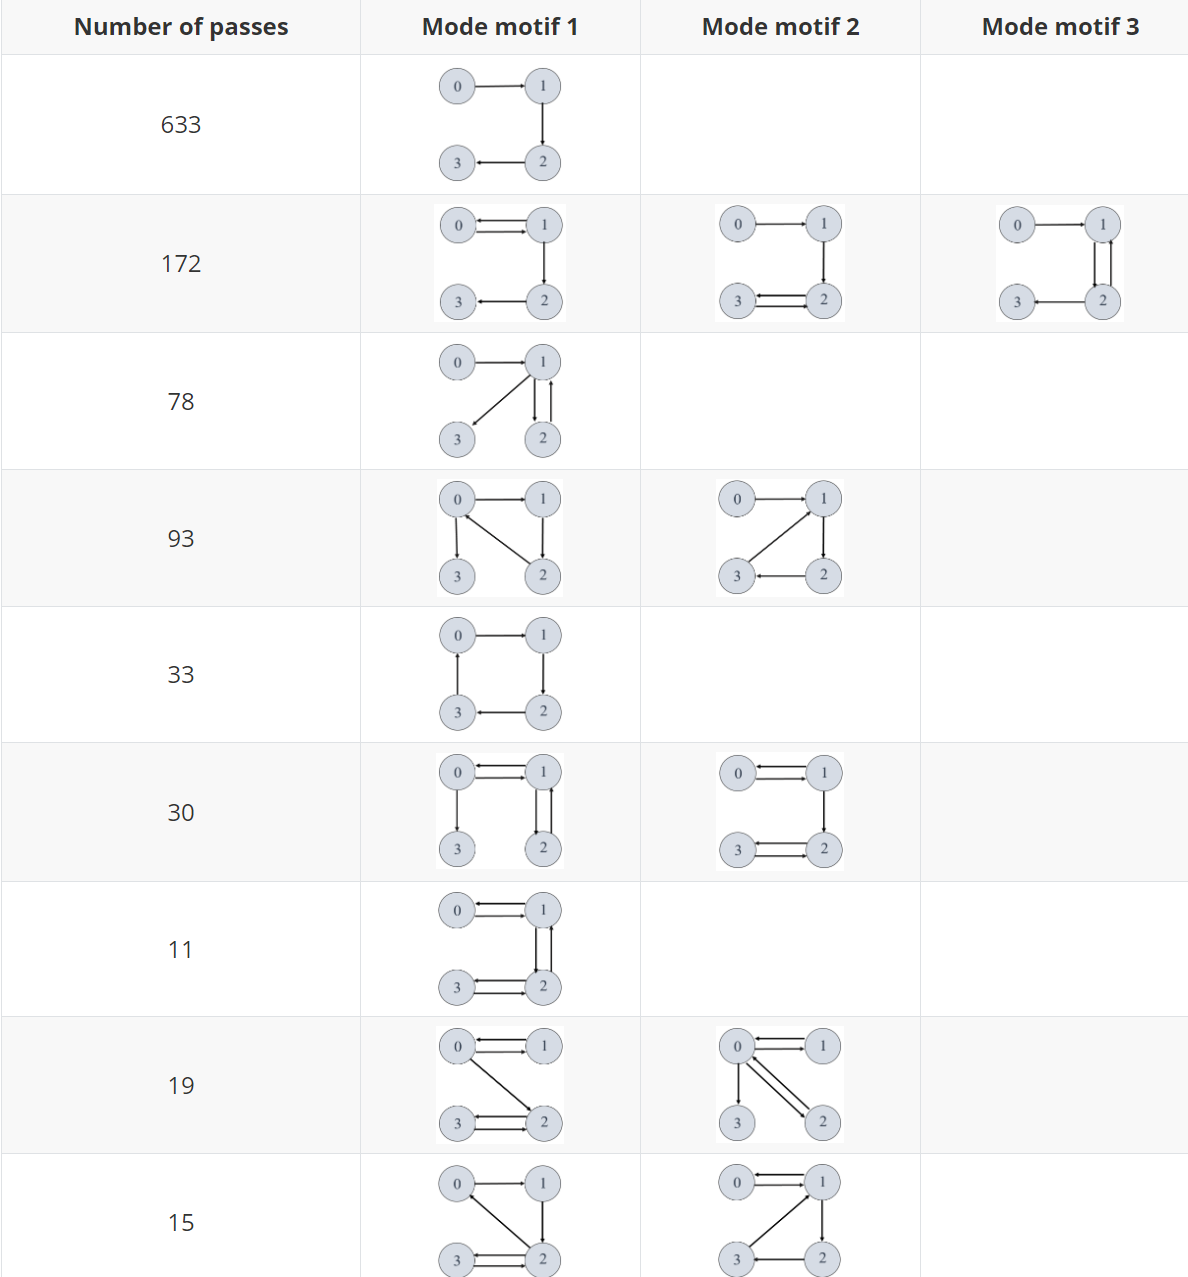
\includegraphics[width=\textwidth]{figures/motif4.png}
	\caption{Mode Motifs for Multiple Configurations}
	\label{fig:motif4}
\end{figure}

\end{appendices}

\end{document}
